\addtocontents{toc}{\protect\newpage}
\chapter{Overzicht spectrum analyzer}
\label{sec:appMapping}
	\begin{figure}[H]
		\centering
		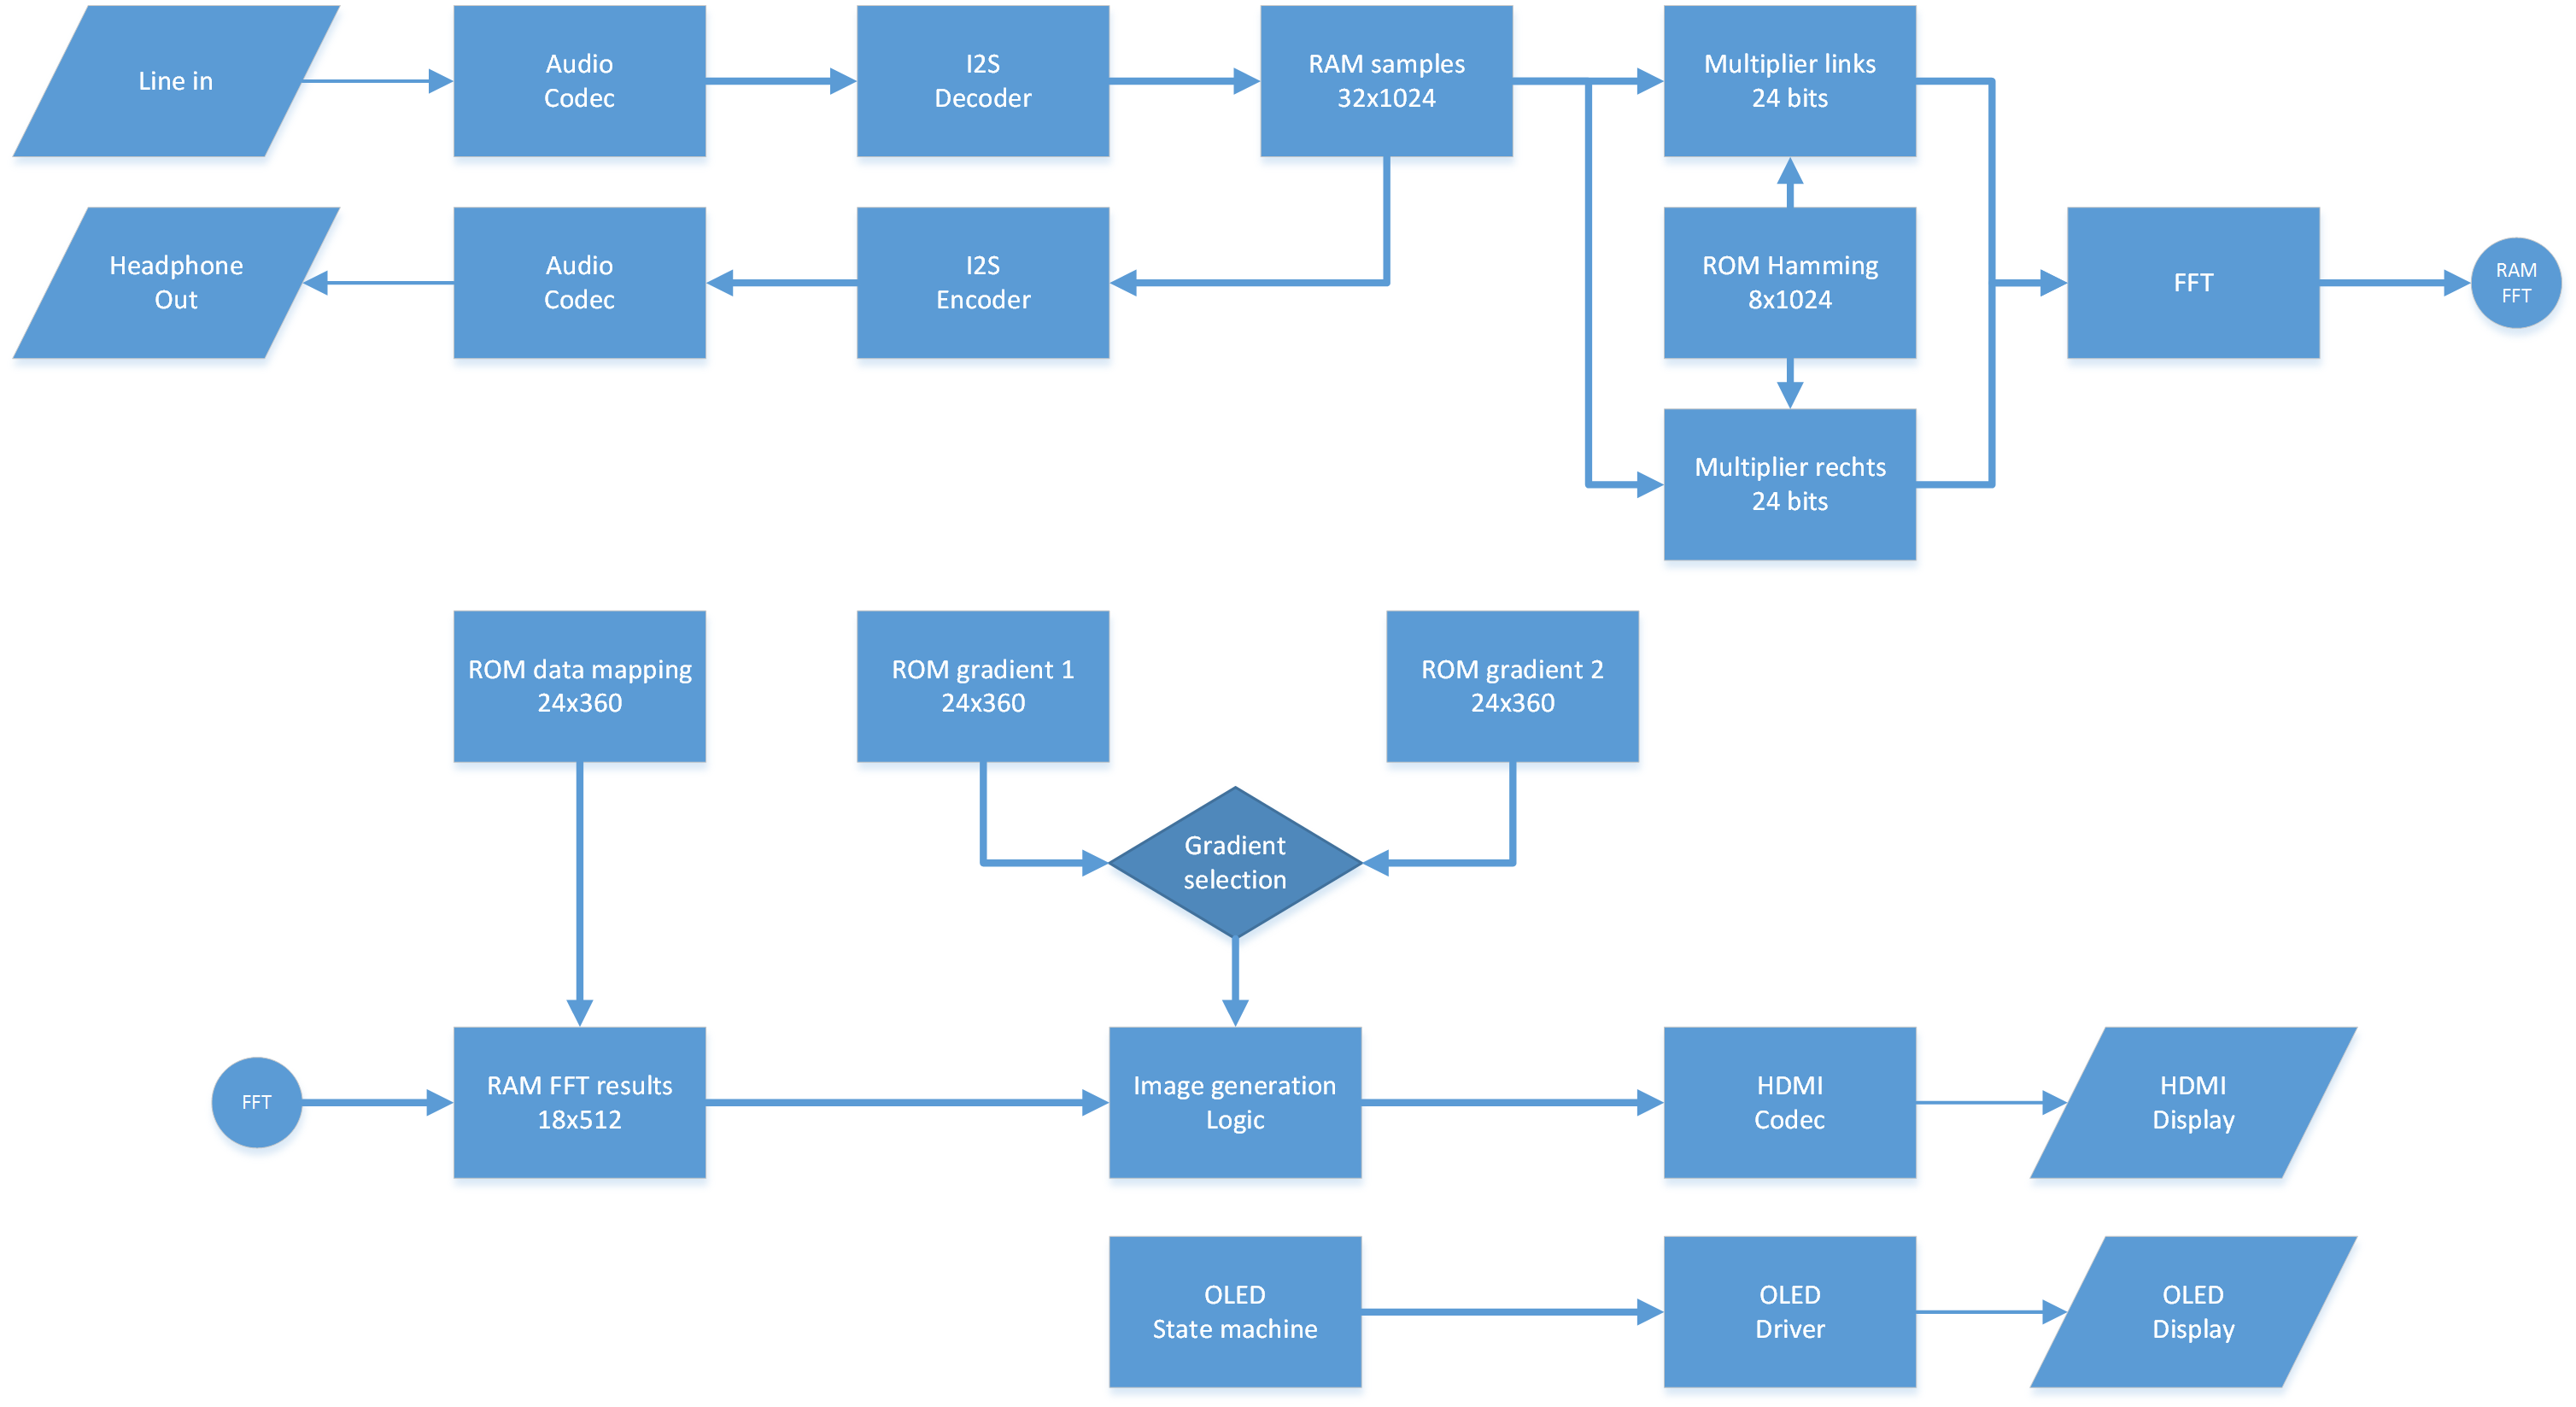
\includegraphics[width=0.75\textheight, angle=270]{Appendix/FlowCharts/Global}
		\caption{Globaal overzicht van de spectrum analyzer}
		\label{fig:FlowChartMapping}
	\end{figure}

\chapter{Componenten}
\section{Top}
\label{sec:appTop}
	\begin{figure}[H]
		\centering
		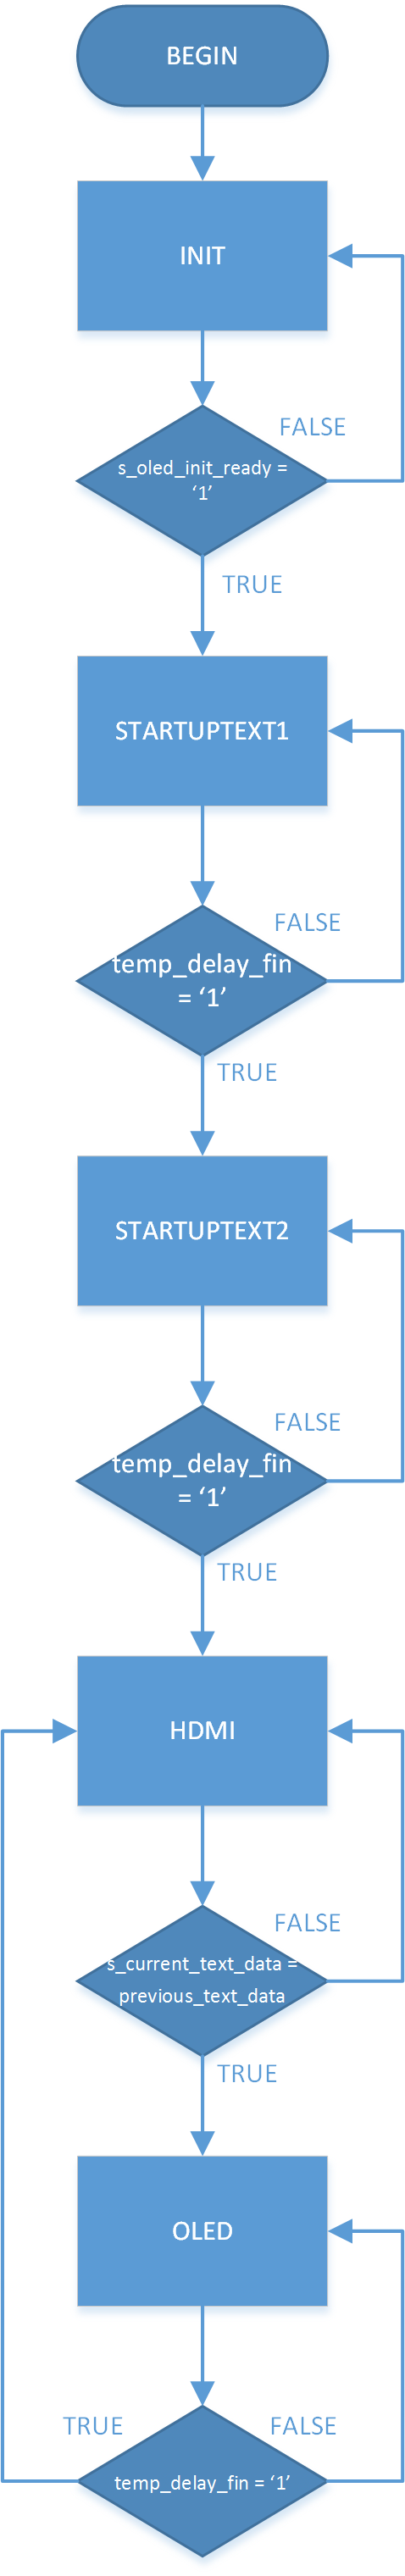
\includegraphics[height=0.66\textheight]{Appendix/FlowCharts/Top}
		\caption{Flowchart van top}
		\label{fig:FlowChartTop}
	\end{figure}

\newpage
\section{Audio interface}
\label{sec:appAudioIf}
	\begin{figure}[H]
		\centering
		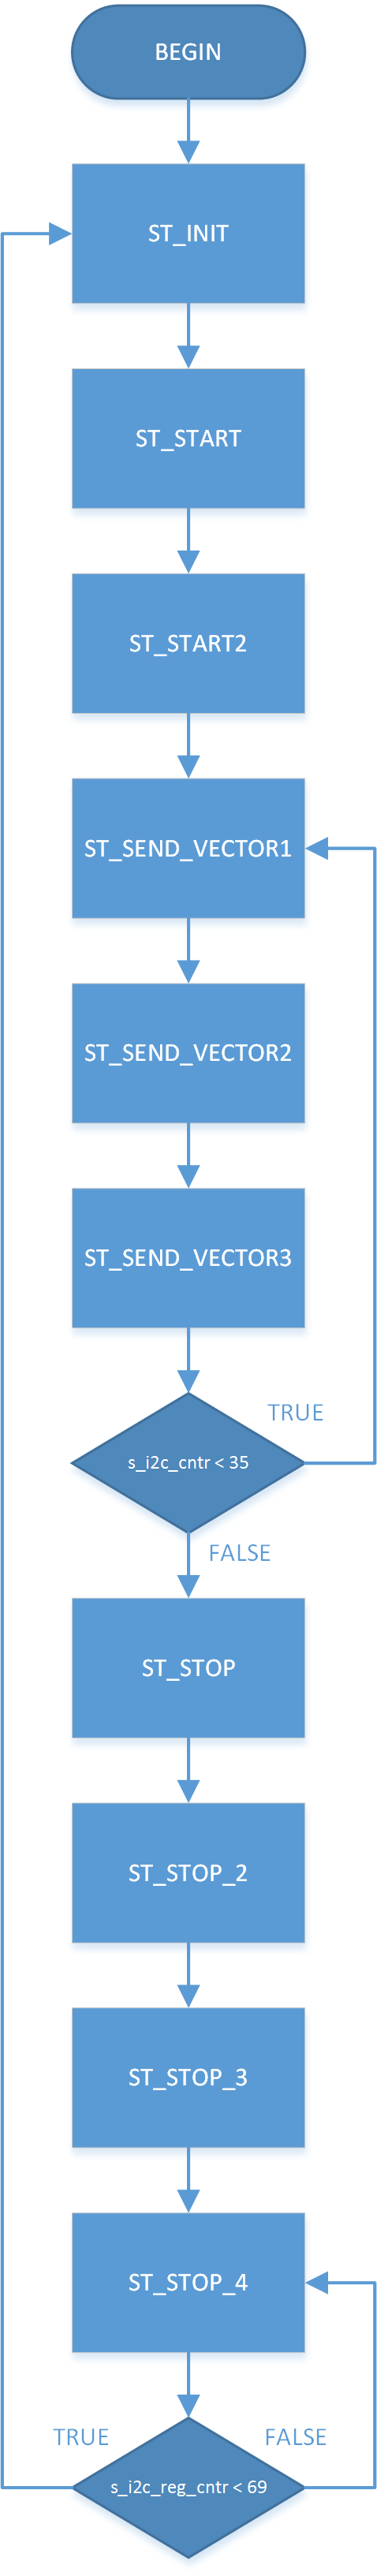
\includegraphics[height=0.85\textheight]{Appendix/FlowCharts/Audio_if}
		\caption{Flowchart van de audio interface}
		\label{fig:FlowChartAudioIF}
	\end{figure}

\newpage
\section{Delay}
\label{sec:appDelay}
	\begin{figure}[H]
		\centering
		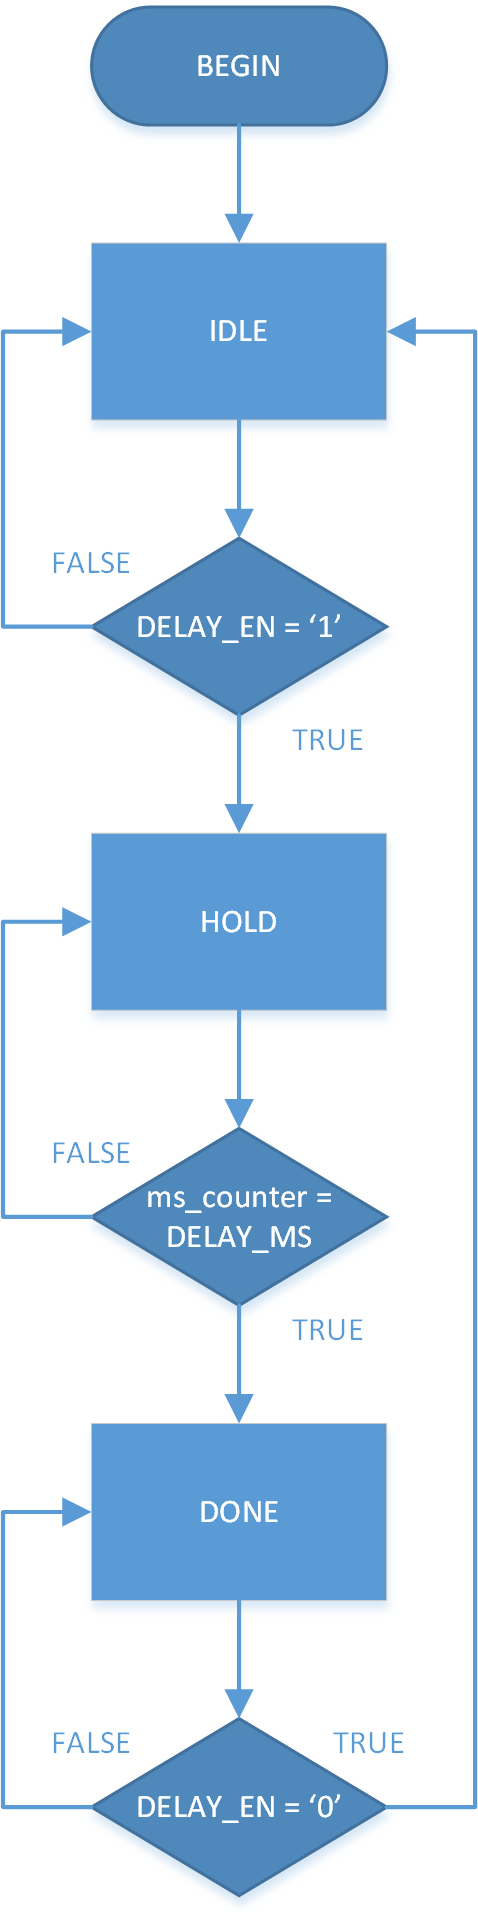
\includegraphics[height=0.85\textheight]{Appendix/FlowCharts/Delay}
		\caption{Flowchart van de audio interface}
		\label{fig:FlowChartDelay}
	\end{figure}

\newpage
\section{Oled top}
\label{sec:appOledTop}
	\begin{figure}[H]
		\centering
		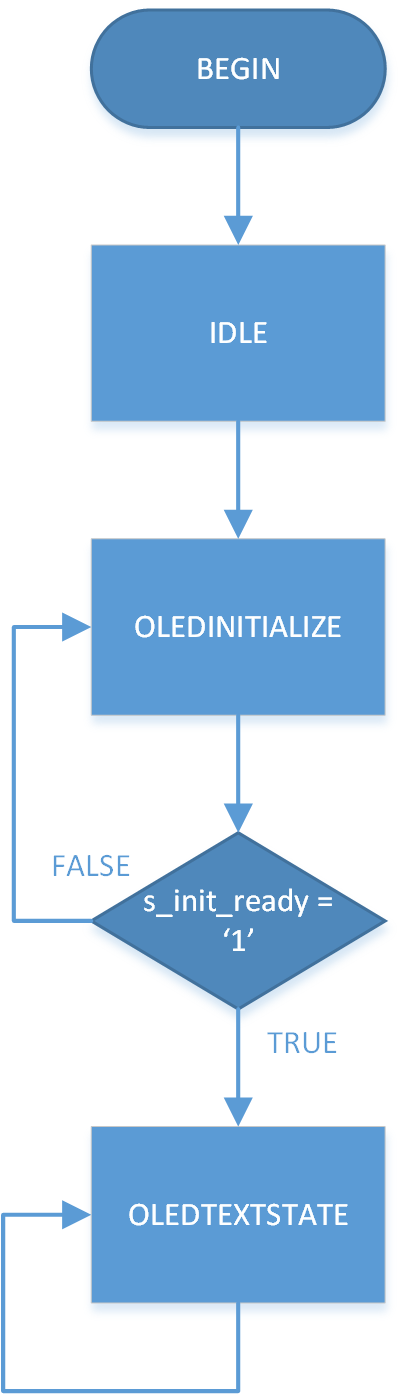
\includegraphics[height=0.85\textheight]{Appendix/FlowCharts/oled_top}
		\caption{Flowchart van oled\textunderscore top}
		\label{fig:FlowChartOledTop}
	\end{figure}

\newpage
\section{Oled initialize}
\label{sec:appOledInit}
	\begin{figure}[H]
		\centering
		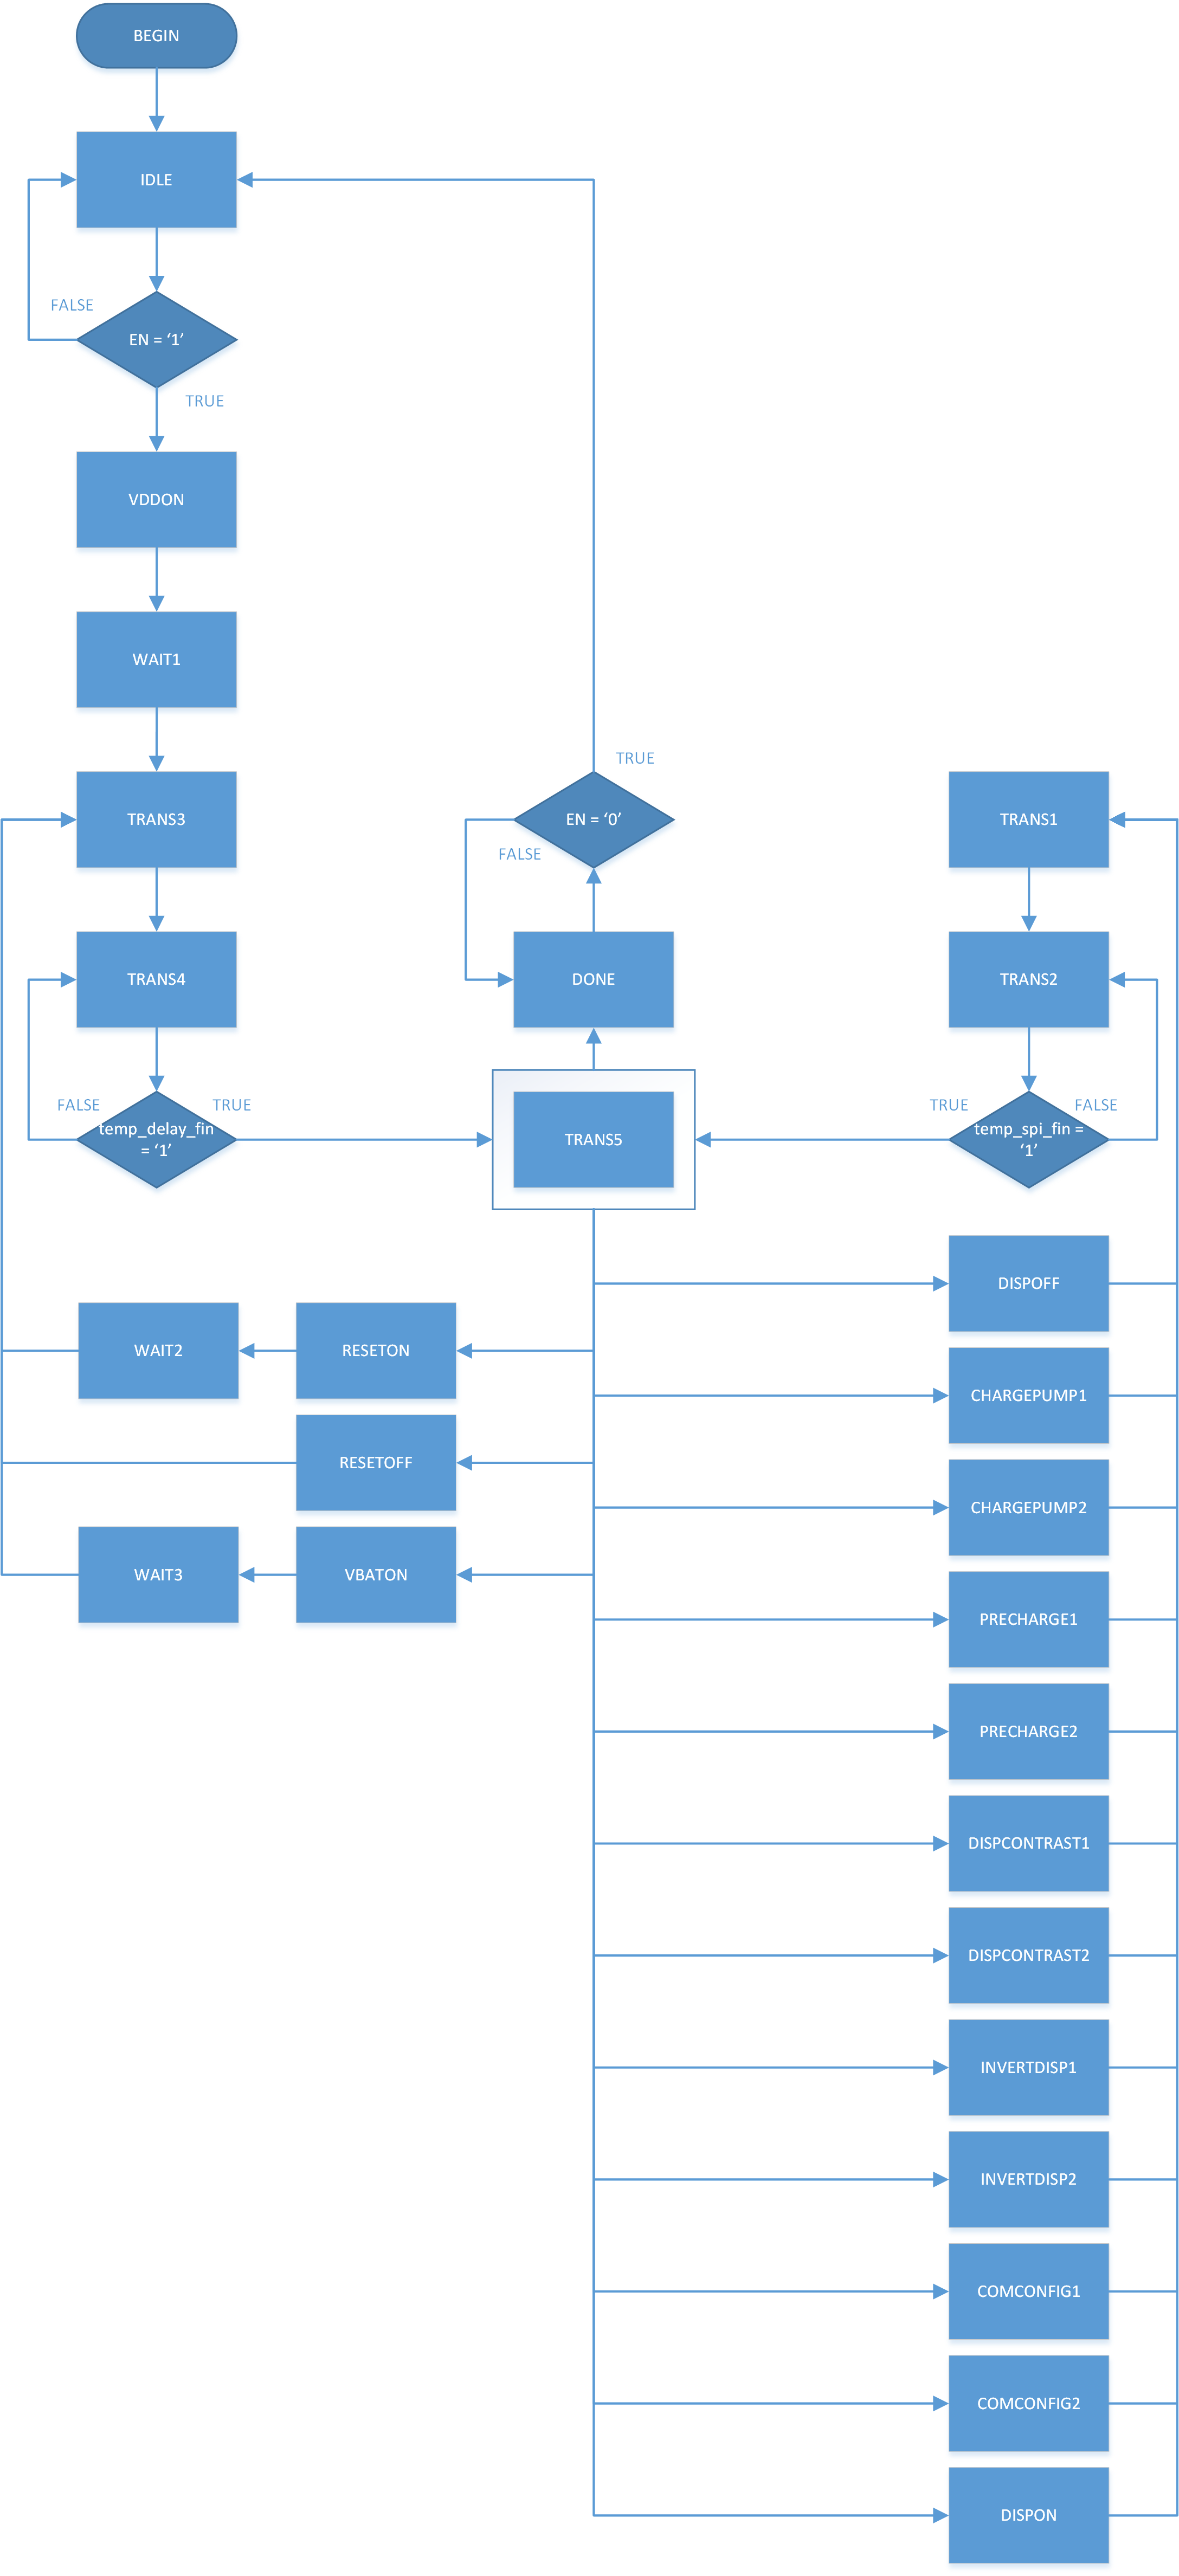
\includegraphics[height=0.85\textheight]{Appendix/FlowCharts/OledInit}
		\caption{Flowchart van OledInit}
		\label{fig:FlowChartOledInit}
	\end{figure}

\newpage
\section{Oled text}
\label{sec:appOledText}
	\begin{figure}[H]
		\centering
		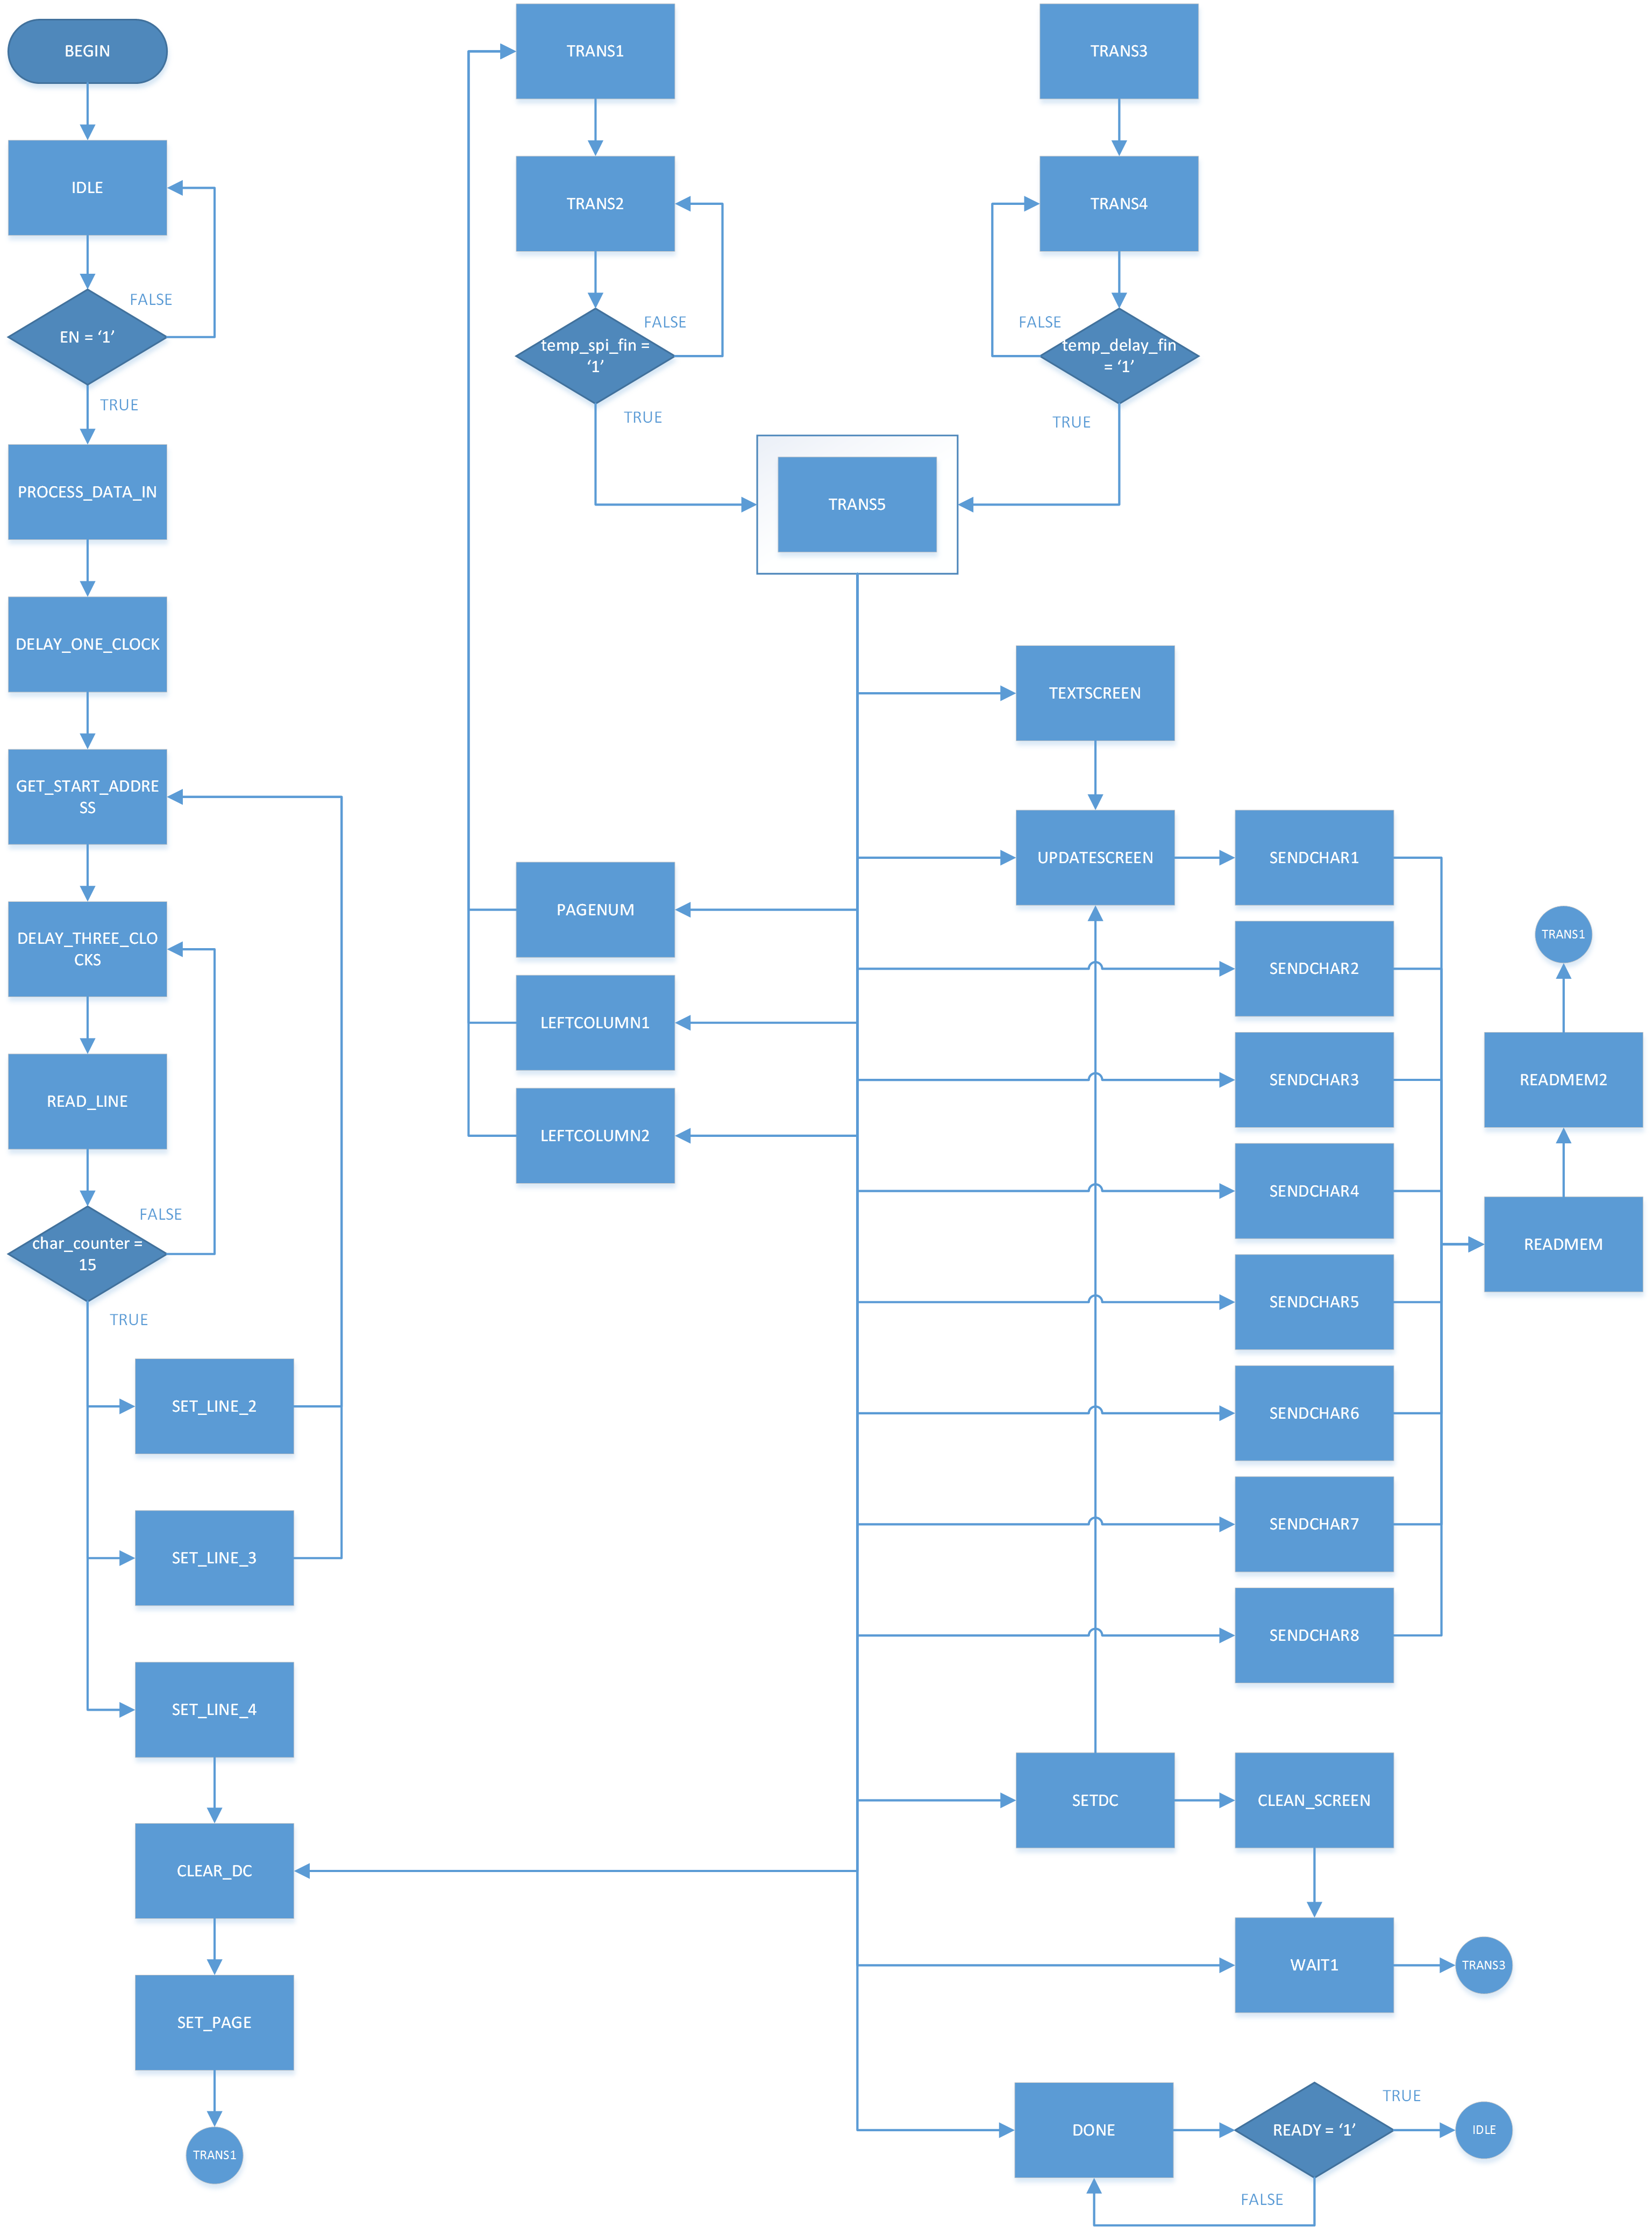
\includegraphics[height=0.85\textheight]{Appendix/FlowCharts/OledText}
		\caption{Flowchart van OledText}
		\label{fig:FlowChartOledText}
	\end{figure}

\newpage
\section{SPI control}
\label{sec:appSpiCtrl}
	\begin{figure}[H]
		\centering
		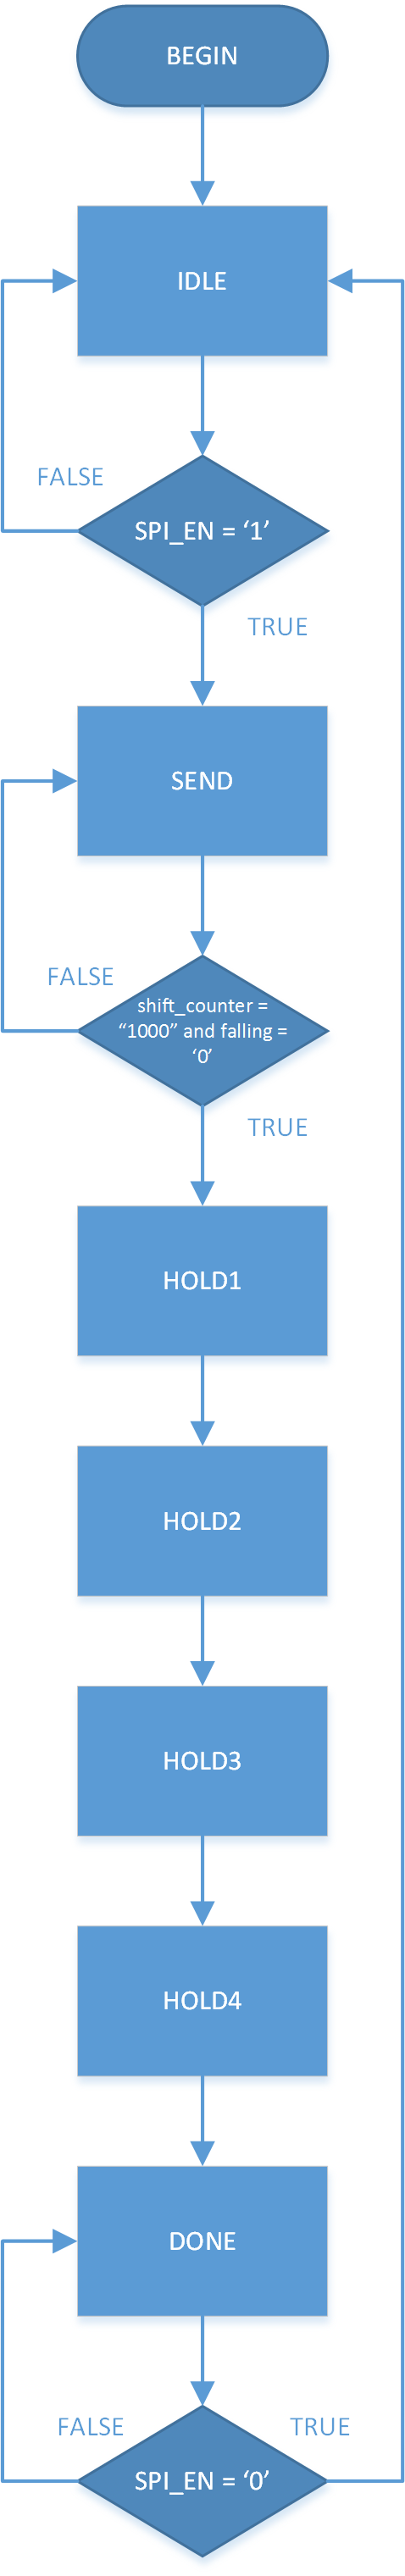
\includegraphics[height=0.85\textheight]{Appendix/FlowCharts/SpiCtrl}
		\caption{Flowchart van SpiCtrl}
		\label{fig:FlowChartSpiCtrl}
	\end{figure}

\chapter{ADAU1761 Settings}
\label{sec:appAdauSettings}
\begin{table}[!htb]
	\footnotesize
    \begin{subtable}{.5\linewidth}
      \centering
        % \caption{}
        \begin{tabular}{l|l}
			Register & Value \\
			\hline
			\hline
			0x4000 & 0x01 \\
			0x4001 & 0x00 \\
			0x4008 & 0x00 \\
			0x4009 & 0x00 \\
			0x400A & 0x01 \\
			0x400B & 0x05 \\
			0x400C & 0x01 \\
			0x400D & 0x05 \\
			0x400E & 0x00 \\
			0x400F & 0x00 \\
			0x4010 & 0x00 \\
			0x4011 & 0x00 \\
			0x4012 & 0x00 \\
			0x4013 & 0x00 \\
			0x4014 & 0x00 \\
			0x4015 & 0x00 \\
			0x4016 & 0x00 \\
			0x4017 & 0x00 \\
			0x4018 & 0x00 \\
			0x4019 & 0x13 \\
			0x401A & 0x00 \\
			0x401B & 0x00 \\
			0x401C & 0x21 \\
			0x401D & 0x00 \\
			0x401E & 0x41 \\
			0x401F & 0x00 \\
			0x4020 & 0x00 \\
			0x4021 & 0x00 \\
			0x4022 & 0x01 \\
			0x4023 & 0xE7 \\
			0x4024 & 0xE7 \\
			0x4025 & 0xE7 \\
			0x4026 & 0xE7 \\
			0x4027 & 0xE7 \\
			0x4028 & 0x00 \\
			\hline
        \end{tabular}
        %\caption{}
    \end{subtable}%
    \begin{subtable}{.5\linewidth}
      \centering
        % \caption{}
        \begin{tabular}{l|l}
			Register & Value \\
			\hline
			\hline
			0x4029 & 0x03 \\
			0x402A & 0x03 \\
			0x402B & 0x00 \\
			0x402C & 0x00 \\
			0x402D & 0xAA \\
			0x402F & 0xAA \\
			0x4030 & 0x00 \\
			0x4031 & 0x08 \\
			0x4036 & 0x03 \\
			0x40C0 & 0x7F \\
			0x40C1 & 0x7F \\
			0x40C2 & 0x7F \\
			0x40C3 & 0x7F \\
			0x40C4 & 0x01 \\
			0x40C6 & 0x00 \\
			0x40C7 & 0x00 \\
			0x40C8 & 0x00 \\
			0x40C9 & 0x00 \\
			0x40D0 & 0x00 \\
			0x40D1 & 0x00 \\
			0x40D2 & 0x00 \\
			0x40D3 & 0x00 \\
			0x40D4 & 0x00 \\
			0x40E9 & 0x10 \\
			0x40EA & 0x00 \\
			0x40EB & 0x7F \\
			0x40F2 & 0x01 \\
			0x40F3 & 0x01 \\
			0x40F4 & 0x00 \\
			0x40F5 & 0x00 \\
			0x40F6 & 0x00 \\
			0x40F7 & 0x00 \\
			0x40F8 & 0x00 \\
			0x40F9 & 0x7F \\
			0x40FA & 0x03 \\
			\hline
        \end{tabular}
        %\caption{}
    \end{subtable}
    \caption{ADAU1761 settings}
\end{table}